%%%%%%%%%%%%%%%%%%%%%%%%%%%%%%%%%%%%%%%%%%%%%%%%%%%%%%%%%%%%%%%%%%%%%%%%%%%%%%%%
%2345678901234567890123456789012345678901234567890123456789012345678901234567890
%        1         2         3         4         5         6         7         8

\documentclass[letterpaper, 10 pt, conference]{ieeeconf}  % Comment this line out
                                                          % if you need a4paper
%\documentclass[a4paper, 10pt, conference]{ieeeconf}      % Use this line for a4
                                                          % paper

\IEEEoverridecommandlockouts                              % This command is only
                                                          % needed if you want to
                                                          % use the \thanks command
\overrideIEEEmargins
% See the \addtolength command later in the file to balance the column lengths
% on the last page of the document

\usepackage{graphicx,graphics}
\usepackage{amssymb,amsmath}
\usepackage{amsfonts}
% \usepackage{calrsfs} % for calligraphic font in math mode
\usepackage{subfigure}
\usepackage{url}
\usepackage{color}
\usepackage{algorithm}
\usepackage{algorithmicx}
\usepackage{algpseudocode}
\usepackage[table,xcdraw]{xcolor}
\usepackage{xargs}[2008/03/08]
\newcommand{\mfcomment}[1]{{\color{blue}[MF: #1]}}
\newcommand{\stcomment}[1]{{\color{blue}[ST: #1]}}


\title{\LARGE \bf
Deep Turtle Control
}

\author{Michael Farrell, Skyler Tolman}
\begin{document}

\maketitle
\thispagestyle{empty}
\pagestyle{empty}

\begin{abstract}
    abstract here
\end{abstract}

%%%%%%%%%%%%%%%%%%%%%%%%%%%%%%%%%%%%%%%%%%%%%%%%%%%%%%%%%%%%%%%%%%%%%%%
% !TEX root=../main.tex
\section{Introduction}
\label{sec:intro}

% A brief introduction to the project.
% Make sure to explain why it's important/relevant/interesting.
% Briefly summarize relevant papers that you build your project on.

Over the past decade, the deep learning revolution has quickly made its way into
many applications and products. During the same time frame, the self-driving car
has rapidly become the focus of many companies ranging from start-ups to tech
giants. It is no mistake that these two movements have gained traction at the
same time. State-of-the-art approaches to the self-driving car problem depend on
a fusion on classical methods with deep
learning~\cite{ramos2017detecting} to create a
reliable solution that can be trusted in a variety of environments.

Though far out of reach with current research, some people believe that the
future of self-driving cars will depend solely on computer vision combined with deep
learning~\cite{huval2015empirical}. This approach attempts to mimic the human
driver, the only example we have to date of a dependable driver in almost any
scenario. As humans, we depend almost entirely on what we perceive with our two
eyes to control the vehicle. This examples leads us to believe that maybe one
day it will be possible to similarly control a vehicle with an end-to-end
approach, with vision as the input and vehicle control as the output.

In the past few years, this simplified approach to the self-driving car problem
has gained traction with hobbyists as well as professionals. NVIDIA's PilotNet
demonstrated the ability of modern convolutional neural networks (CNNs) to map
raw pixels from a single front-facing camera directly to steering
commands~\cite{bojarski2016end}. NVIDIA was also able to show that PilotNet's steering
command output was affected most by visual cues in the images that human drivers
also react to including lane lines, parked cars, and unexpected
obstacles~\cite{bojarski2017explaining}. Hobbyists have applied a similar
approach to create autonomous, remote control
cars~\cite{bechtel2018deeppicar}~\cite{donkeycar}.

The principle of end-to-end control has been seen in a variety of applications.
For deep visuomotor policies, such as a robot arm picking up an object, it has
even been shown that training the perception and control systems jointly
end-to-end provides better performance than training each component
separately~\cite{levine2016end}.

In this work, we develop and test an end-to-end control method for a TurtleBot
robot (Figure \ref{fig:turtlebot_pic}) following a course created from a pair of
ropes. To simplify the problem, we command a constant desired linear velocity
for the Turtlebot and focus only on controlling the steering.
As in NVIDIA's PilotNet, our method uses
individual camera images to predict the steering command for the robot. Other
similar work has shown that recurrent neural networks, such as those using an
LSTM~\cite{xingjian2015convolutional}, have the ability to learn both the visual
and dynamic temporal dependencies of a self-driving vehicle~\cite{eraqi2017end}.
Additionaly, methods that use a video stream as the input as opposed to
still-frame images have shown the ability to learn spatiotemporal
features~\cite{tran2015learning}. Though these approaches may be great, natural
extensions of this work, we describe a basic, easy-to-implement method that
extends to a variety of ground robot tasks.

This paper describes our approach in the following manner. Section
\ref{sec:classical} describes an end-to-end control formulation using classical
methods of image processsing and control. Section \ref{sec:network} describes an
end-to-end control formulation using a deep neural network.
Section~\ref{sec:results} describes the results of our experiments including the
advantages and disadvantages of the classical and neural network based
approaches. Section~\ref{sec:future_work} provides some concluding remarks and
some suggestions for future work.

%Nvidia PilotNet. Finding the salient objects that contribute to the output.
%Shows that it learned to look at lane lines, sides of roads, cars parked on the
%side, etc.~\cite{bojarski2017explaining}.

%End to end for deep visuomotor policies. Learn visuomotor polies to control the
%torque of a robot arm to do basic tasks like place a hanger, pick up objects.~\cite{levine2016end}.

%Learn spatiotemporal features. Used in video such as action recognition.~\cite{tran2015learning}

%LSTM for RNN.~\cite{xingjian2015convolutional}

%Attempt to learn both visual and dynamic temporal dependencies of driving with
%an RNN. Trained on comma.ai dataset. C-LSTM outperforms CNN.~\cite{eraqi2017end}

%Small scale version of Nvidia's PilotNet running on a Raspberry Pi.~\cite{bechtel2018deeppicar}

%Donkeycar also.~\cite{donkeycar}.


\begin{figure}
  \centering
  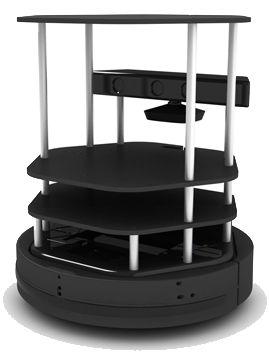
\includegraphics[scale=1.5]{figures/turtlebot.png}
  \caption{TurtleBot robot used in experiments.}
  \label{fig:turtlebot_pic}
\end{figure}


% !TEX root=../main.tex
\section{Classical Approach}
\label{sec:classical}

In an effort to better understand the vision problem presented, we first
describe a classical approach to the TurtleBot control problem. Implementation
of the methods described here was done in C++ using the OpenCV
library~\cite{opencv_library}. As described above, we seek to control the
TurtleBot robot through a track outlined with a pair of white ropes. The
commanded control of the robot must only depend on the current image from the
camera mounted on the robot.

Figure~\ref{fig:raw_img} shows an example image from the camera mounted on the
TurtleBot. As seen in this image, the lower quarter of the image is taken up by
the robot itself, effectively providing no useful information to control from.
Based on experimentation, at the constant velocity of 0.3 $m/s$ used for our
experiments, the top section of the image also does not provide any relevant
information for the current control. For these reasons, we first crop out the top
and bottom of the image to produce an image like that seen in 
Figure~\ref{fig:classical_crop}.

The first step in the classical end-to-end control approach is to detect the
ropes in the camera image. As the ropes do not change color, we employ a simple
segmentation method based on color. To segment the white color of the ropes, we
transform the image from RGB color space to HLS (Hue Lightness Saturation)
color space. The color white is found in the HLS space at any values for hue and
saturation with a high value for lightness. Using this knowledge, we create a
mask of the targeted color, white, using a threshold value on the lightness
value of each pixel. The result of this method is a binary mask as seen in
Figure~\ref{fig:classical_thresh}.

The second step of the classical approach is to locate and classify the left
rope and the right rope. In an ideal scenario, such as that depicted in
Figure~\ref{fig:classical_thresh}, this is as simple as detecting the two
largest contours in the binary mask and classifying the left contour as the left
rope and the right contour as the right rope. If no contour is detected on
either side, we declare that particular rope to be out of the field of view of
the camera. Classifying the ropes becomes
ambiguous in scenarios such as that depicted in Figure~\ref{fig:classical_fail}
when the rope is seen lengthwise across the image. This is the major downfall of
an end-to-end approach using only the current camera image. When the robot
approaches a sharp turn or gets into a bad configuration, the camera image can
appear like Figure~\ref{fig:classical_fail} where there is no clear direction
for the robot to follow.

After rope detection and classification, we must compute a steering command. To
compute the desired steering command, we first fit a second-order spline to each
of the detected ropes as seen in Figure~\ref{fig:classical_fit}. This spline
fitting serves to smooth out the desired path to follow. We evaluate each spline
at a given height in the image, near the top of the cropped image. We then
average these spline evaluations to get an approximate for our location between
the ropes. We then multiply the error between the average of these spline
evaluations and the center of the image by a proportional gain to get the
desired angular velocity of the TurtleBot.

\begin{figure}
  \centering
  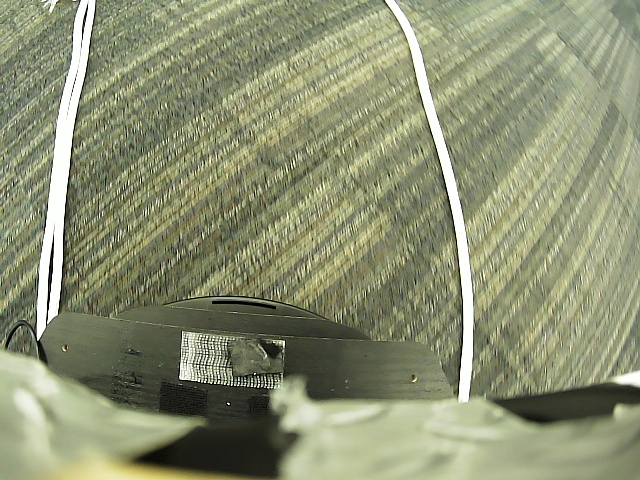
\includegraphics[scale=0.5]{figures/raw_img.png}
  \caption{Example image from the camera mounted on the TurtleBot.}
  \label{fig:raw_img}
\end{figure}

\begin{figure}
  \centering
  
\includegraphics[scale=0.67]{figures/classical_crop.jpg}
  \caption{Cropped image from TurtleBot.}
  \label{fig:classical_crop}
\end{figure}

\begin{figure}
  \centering
  
\includegraphics[scale=0.5]{figures/classical_thresh.jpg}
  \caption{TurtleBot image mask after thresholding.}
  \label{fig:classical_thresh}
\end{figure}

\begin{figure}
  \centering
  
\includegraphics[scale=0.5]{figures/classical_contours.jpg}
  \caption{TurtleBot image mask with only the largest contours.}
  \label{fig:classical_contours}
\end{figure}

\begin{figure}
  \centering
  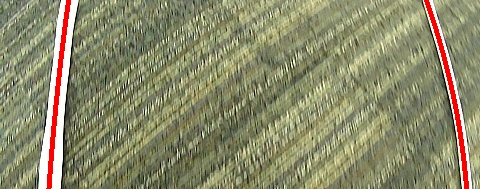
\includegraphics[scale=0.5]{figures/classical_fit.jpg}
  \caption{TurtleBot image with splines fit to largest contours.}
  \label{fig:classical_fit}
\end{figure}

\begin{figure}
  \centering
  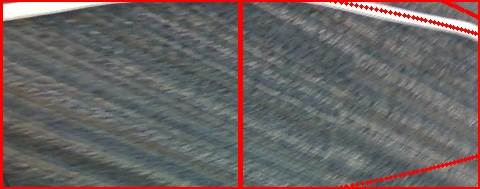
\includegraphics[scale=0.5]{figures/classical_fail.jpg}
  \caption{Example of a failure mode of the classical end-to-end control method.}
  \label{fig:classical_fail}
\end{figure}


% !TEX root=../main.tex
\section{Network Approach}
\label{sec:network}
The end goal of our project was to get the turtlebot to follow a track purely using an image input to a neural network.
This section describes the architecture and training methods used to train a control network for the turtlebot.

\subsection{Network architecture}
We experimented with multiple architectures, including a simple convolutional neural network (CNN), and a ResNet~\cite{ResNet}, but we eventually decided to use the DenseNet as our base architecture~\cite{DenseNet}.

\begin{figure}[hbt]
  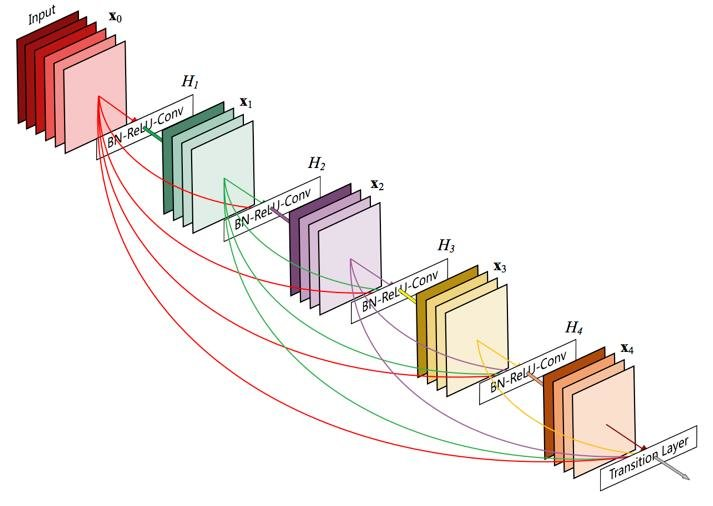
\includegraphics[width=\columnwidth]{figures/densenet}
  \caption{DenseNet architecture}
  \label{fig:densenet}
\end{figure}

The Densenet is an network architecture with densely connect convolutional blocks, as seen in Figure~\ref{fig:densenet}. The DenseNet architecture is unique because of the densely connected skip connections across multiple convolutional blocks, which allows the architecture to re-use features throughout the network. Accordingly, it has achieved better results on benchmarks such as ImageNet with a smaller memory footprint.

We used a pre-trained model for the DenseNet convolutional blocks, and added three linear layers with dropout to train the turtlebot control using the DenseNet features.

\subsection{Network Training}
We used supervised "imitation" learning to train the control network. We collected data by driving the turtlebot around multiple tracks on different ground surfaces and matched RGB camera images to angular velocity command outputs. We initially used the classical vision control method to gather data on a single track, then diversivied the data by manually driving the turtlebot around other varied tracks and surfaces.

Using the image-command pairs, we trained the neural network to predict the appropriate command for each input image. We trained the network on about 7 epochs of 15,000 images.

\subsection{Continous Control}
Ideally, we would like the network to be able to predict a continous control output given an input image. We allowed the network output to range from -1 to 1 radians per second. A simple way to limit the control effort was to use a hyperbolic tangent function as the final activation on our linear layer backend.

After multiple attempts at training the network to predict a continouous output, we were able to get some success, but the turtlebot had a hard time making sharper turns and would often drive straight off the course instead of making the turns. In general, the control was underactuated.

\begin{figure}[hbt]
  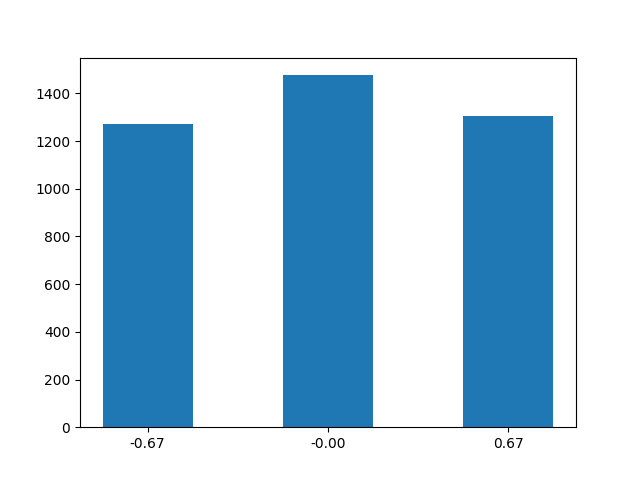
\includegraphics[width=\columnwidth]{figures/data_histogram}
  \caption{Histogram of the omega commands for the training data used.}
  \label{fig:data_hist}
\end{figure}

We assume that the issue was a data problem, so we plotted a rough distribution of the data, as seen in Figure~\ref{fig:data_hist}. The data is centered about mean and has a larger proportion of commands close to zero than it does further away. It seems as though the network was able to quickly decrease the loss by driving the control close to zero, causing the turtlebot to default to slower angular rates. The problem was then magnified because the turtlebot would fail to turn sharply and place itself in a situation that it had not seen before and could not recover from.

To overcome this issue, we decided to try using an architecture with discrete outputs and treat it as a classification problem. Some other potential solutions to our problems could have included augmenting the data to include more off-center scenarios or to gather data with more variety, including the corner cases where the turtlebot needs to recover from poor control or poor initial conditions.

\subsection{Discretized Control}
As a simple solution to the difficulties we faced when using continous control, we decided to discretize the control by binning the allowable omega values and using the midpoint of each bin as the representative omega value for that bin. We used 5 bins to keep the classification problem simple, but still have enough control authority to navigate sharper turns. With five bins, the allowable control outputs were -0.8 (hard left), -0.4 (left), 0.0 (straight), 0.4 (right), and 0.8 (hard right). Neural networks are often better suited to classification problems and by using a cross-entropy loss function instead of the mean squared error loss we had used for the continous output, the network lost the incentive to center commands near zero, but instead was required to classify each image in the correct command bin.

This approach proved to be much more successful and we were able to replicate and eventually surpass the performance of the classical method.


% !TEX root=../main.tex
\section{Results}
\label{sec:results}

We were pleased to be able to succesffully implement autonomous control of a
TurtleBot using an end-to-end visual control approach. The classical approach served as a meaningful learning experience and also a useful tool in collecting data to train the neural network approach, which was our end goal.

\begin{figure}[hbt]
  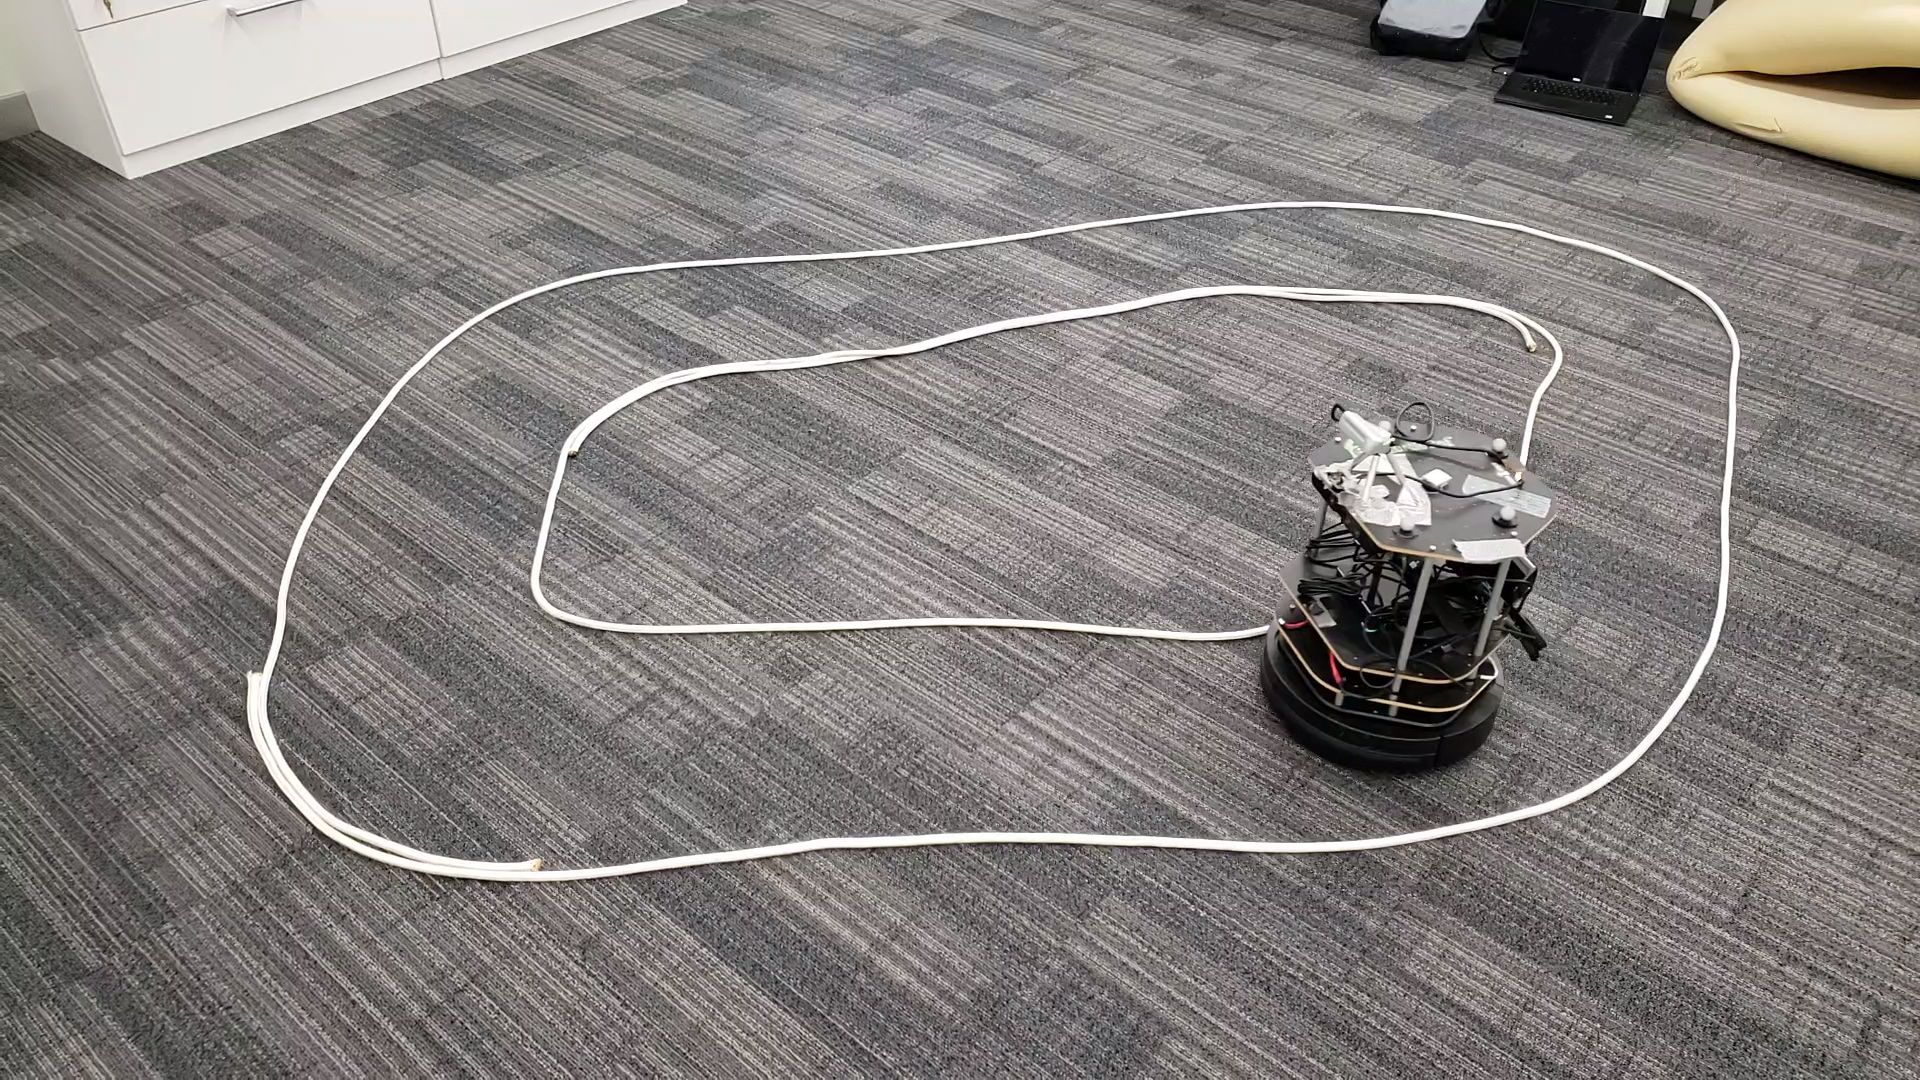
\includegraphics[width=\columnwidth]{figures/success_track}
  \caption{Snapshot of the TurtleBot successfully following a track using end-to-end deep learning-based control.}
  \label{fig:success_track}
\end{figure}

Some of the main advantages we saw of using the neural network control as opposed to the classical method was the ability to implicitly encode variability and robustness into the control simply by training on more data in varied environments. For example, the classical method, which depended heavily on proper segmentation, needed to be re-tuned for each ground surface and lighting condition, whereas the neural network was able to learn how to extract the proper features in multiple environments without the need to explicitly retune or revise the network.

It was also interesting to note the information the neural network was able to
learn. To visualize the salient features in a given image, we evaluated the
gradient of the output of the network with respect to the input image at the
given image. We then normalized these gradeints to turn them into a visible
grayscale image, equal in size to that of the input image. As seen in
Figures~\ref{fig:saliency1}~through~\ref{fig:saliency3}, the brightest pixels in
the gradient images correspond to the pixels that most contributed to the output
of the neural network. For the most part, these salient pixels correspond to the areas where the rope is seen in the input image. Note how the neural network learned to identify the rope specifically, not just white objects, as the light reflection in Figure~\ref{fig:saliency3} is filtered out and does not contribute much to the output. These glare spots were difficult for the classical method to handle, which conveys a clear advantage of the network-based control over the classical control.

\begin{figure}[hbt]
  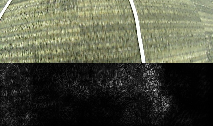
\includegraphics[width=\columnwidth]{figures/saliency1}
  \caption{Top: Original image; bottom: Class saliency for rope on carpet data. Shows the gradient is highest near where the rope appears in the original image (top)}
  \label{fig:saliency1}
\end{figure}

\begin{figure}[hbt]
  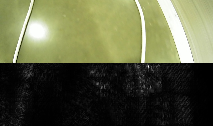
\includegraphics[width=\columnwidth]{figures/saliency2}
  \caption{Class saliency on reflective concrete flooring.}
  \label{fig:saliency2}
\end{figure}

\begin{figure}[hbt]
  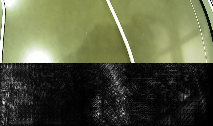
\includegraphics[width=\columnwidth]{figures/saliency3}
  \caption{Class saliency on reflecitve concrete floor with mulptiple glare spots. Show that the network learned to filter out bright contours that do not correspond with rope.}
  \label{fig:saliency3}
\end{figure}


% !TEX root=../main.tex
\section{Future Work}
\label{sec:future_work}
Although the control was sufficient to navigate a simple track multiple times, there is definitely room for improvement. One main disadvantage of our current method is that the discretized cotrol is somewhat jerky and it could potentially limite the robots ability to make sharper turns on more difficult tracks if the avaiable discrete values were insufficient to make the turn. Some possible improvements to overcome this could be to use more bins to better approximate continuous control, or possibly to better collect and augment the data used to train the continous control output to see if we can produce effective control without discretization.

We would also like to find ways to extend the results of this project beyond the contrived example of following rope lanes to something with real-world usefulness. This could include training the network to use more natural features to navigate such as hallways, aisles, existing tile markings, or sidewalks. This would allow the network to leverage it's full potential to interpret high level features rather than just simple lines. Another extension that could improve the usefulness of this control method could be to integrate the autonomous control with SLAM (simulataneous localization and mapping) or some other mapping algorithm to not only navigate the real world, but also to collect data about the environment along the way.

This turtlebot control project proved to be a useful opportunity for us to apply deep learning and computer vision principles to a non-trivial problem and to gain some real-world experience implementing these technologies on a hardware platform.




%%%%%%%%%%%%%%%%%%%%%%%%%%%%%%%%%%%%%%%%%%%%%%%%%%%%%%%%%%%%%%%%%%%%%%%
\bibliographystyle{IEEEtran}
\bibliography{library}

\end{document}
